\documentclass[12pt]{standalone}
\usepackage[utf8]{inputenc}
\usepackage[T1]{fontenc}
\usepackage{times}
\usepackage{amsmath,amssymb}
\usepackage[dvipsnames,svgnames]{xcolor}
\usepackage{tikz}
\usetikzlibrary{decorations.pathreplacing, calc, positioning, shapes.geometric, shapes.symbols, arrows.meta, backgrounds, fit, shapes.misc}
\definecolor{RED}{rgb}{1,0,0}
\definecolor{dmrsfill}{HTML}{CDE2FB}
\definecolor{winblue}{HTML}{0D366B}
\definecolor{inksec}{HTML}{52514E}
\begin{document}
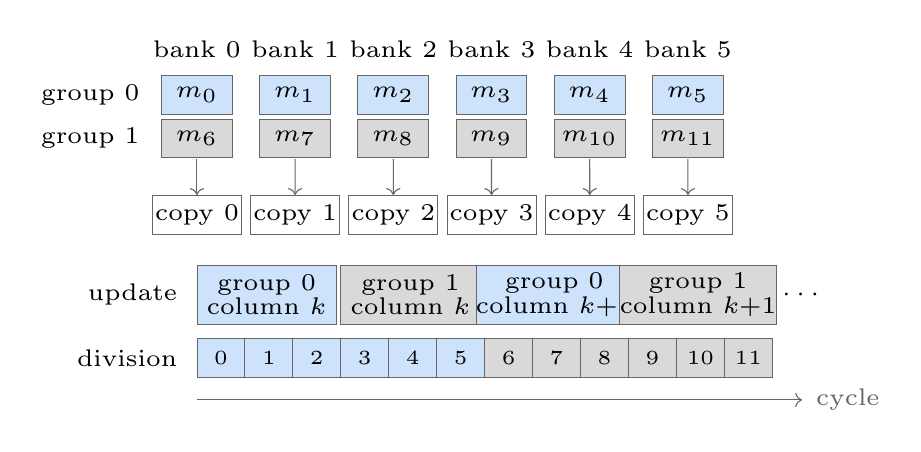
\begin{tikzpicture}[scale=1.45, transform shape, font=\fontsize{6.5}{7.8}\selectfont,
  mat/.style={draw=black!60, fill=#1, minimum width=0.62cm, minimum height=0.34cm, inner sep=0pt, line width=0.3pt},
  via/.style={draw=black!60, fill=white, minimum width=0.78cm, minimum height=0.34cm, inner sep=0pt, line width=0.3pt}]
\def\u{0.86}
\definecolor{g0}{HTML}{CDE2FB}\definecolor{g1}{HTML}{D9D9D9}
% bancos: matriz m no banco m mod 6
\foreach \p in {0,...,5} {
  \pgfmathtruncatemacro{\q}{\p+6}
  \node at (\p*\u, 0.40) {bank \p};
  \node[mat=g0] at (\p*\u, 0) {$m_{\p}$};
  \node[mat=g1] at (\p*\u, -0.38) {$m_{\q}$};
  \node[via] (v\p) at (\p*\u, -1.05) {copy \p};
  \draw[black!60, ->, line width=0.4pt] (\p*\u, -0.56) -- (v\p.north);
}
\node[left] at (-0.38, 0) {group 0};
\node[left] at (-0.38, -0.38) {group 1};
% ciclos do laço de atualização
\begin{scope}[shift={(0,-1.75)}]
\foreach \c/\g/\k/\cor in {0/0/k/g0, 1/1/k/g1, 2/0/k{+}1/g0, 3/1/k{+}1/g1} {
  \node[mat=\cor, minimum width=1.22cm, minimum height=0.52cm, align=center, font=\fontsize{6}{7}\selectfont] at (\c*1.26+0.61, 0) {group \g\\[-1pt]column $\k$};
}
\node[left] at (-0.05, 0) {update};
\node[right] at (5.0, 0) {$\cdots$};
\foreach \c in {0,...,11} {
  \pgfmathtruncatemacro{\gg}{\c<6 ? 0 : 1}
  \ifnum\gg=0 \def\cc{g0}\else\def\cc{g1}\fi
  \node[mat=\cc, minimum width=0.42cm] at (\c*0.42+0.21, -0.55) {\fontsize{5.5}{6}\selectfont\c};
}
\node[left] at (-0.05, -0.55) {division};
\draw[black!60, ->, line width=0.4pt] (0,-0.92) -- (5.3,-0.92) node[right] {cycle};
\end{scope}
\end{tikzpicture}
\end{document}
